% Chapter 2 - Background

\glsresetall % reset the glossary to expand acronyms again
\chapter[Literature Review]{Literature Review}\label{ch:LitReview}
\index{Literature Review}

%What to expact in this chapter

This chapter provides a comprehensive evaluation of literature relevant to the research topic. It begins with an introductory section outlining the motivation for the study, focusing on the need to further investigate mobile app development for digitising and storing ECG paper records. A brief overview of the theory behind ECG signal formation follows, providing the foundation for understanding its digitisation. 

The review then adopts a funnel approach: first examining existing methods of ECG record digitisation, then evaluating the potential of mobile applications for this purpose through image capture, and finally considering techniques for extracting ECG waveforms from images. The chapter concludes with a summary of key findings, identifying gaps in current research and setting the stage for the methodology that follows.

%----------------------------------------------------------------------------------------------

\section{Introduction}

The electrocardiogram (ECG) has been a fundamental tool in medicine since 1901 \cite{MartinezPerez2013MobileAppsCardiology}. Over the years, a vast number of ECG paper records have been produced. Consequently, researchers have devised methods to digitise these records in order to ensure long-term preservation, improve accessibility, and facilitate future evaluation and diagnosis. It is therefore important to investigate and assess these methods to understand their respective strengths and limitations.

With the growing use of mobile applications in healthcare \cite{Steinhubl2013CanMHealth}, new opportunities for ECG digitisation have emerged. This enables investigation into whether ECG images captured with mobile devices can be effectively processed for digitisation.

%----------------------------------------------------------------------------------------------

\section{ECG Fundamentals} \label{sec: ECG_Fund}
% the problem with this section is that it doesn't add points to delebarate over - how advantageous or disadvantageous or how the results sway the decsions

Electrocardiogram signals show how the path of the \gls{depolarization wave} - the flow of a group of positive electric charges - moves during each heartbeat \cite{osmosisECGbasics2025}. Hearts have natural pacemakers that initiate electric signals that cause atrial and ventricular contraction \cite{myhealthSAnode2024}. Electrocardiograms are built to sense these natural signals and convert them into useful information that portray the heart's condition.

\subsection{ECG Signal Generation}

The electric activity of the heart is governed by the sinoatrial (SA) and atrioventricular (AV) nodes. The SA node initialises the impulses and the AV node introduces delays to their delivery to co-ordinate between arterial and ventricular contractions for optimum heart functionality \cite{myhealthSAnode2024}.

As the positive charges move through the heart's muscles, their negative resting state changes to a positive active state. This change in charge of the internal muscles affects a change to the external charge surrounding it \cite{osmosisECGbasics2025}. This creates the potential difference measured by the electrocardiogram electrodes. If detected it is noted as a deflection on the ECG waveform. The bigger the potential difference, the larger the deflection \cite{osmosisECGbasics2025}.

(image explaining or showing ECG deflections - so they know what to look for in the actual trace)

\subsection{ECG Waveform Formation}

An ECG signal consists of five deflections that together form the PQRST complex, representing a single heartbeat and the complete cycle of myocardial contraction and relaxation \cite{AlGhatrif2012}.

The P wave reflects atrial depolarisation, initiating atrial contraction. It is typically a low-amplitude, gently sloped deflection due to the slower propagation of the depolarisation wave through atrial myocardial cells \cite{OReilly2023ModelDrivenAO}. The QRS complex corresponds to ventricular depolarisation and the onset of ventricular contraction, with the R wave being the largest positive deflection \cite{Prima2018PolyanilineAN}. The T wave represents ventricular repolarisation, preparing the ventricles for the next cardiac cycle \cite{Prima2018PolyanilineAN}.

\begin{figure}[H]
    \centering
    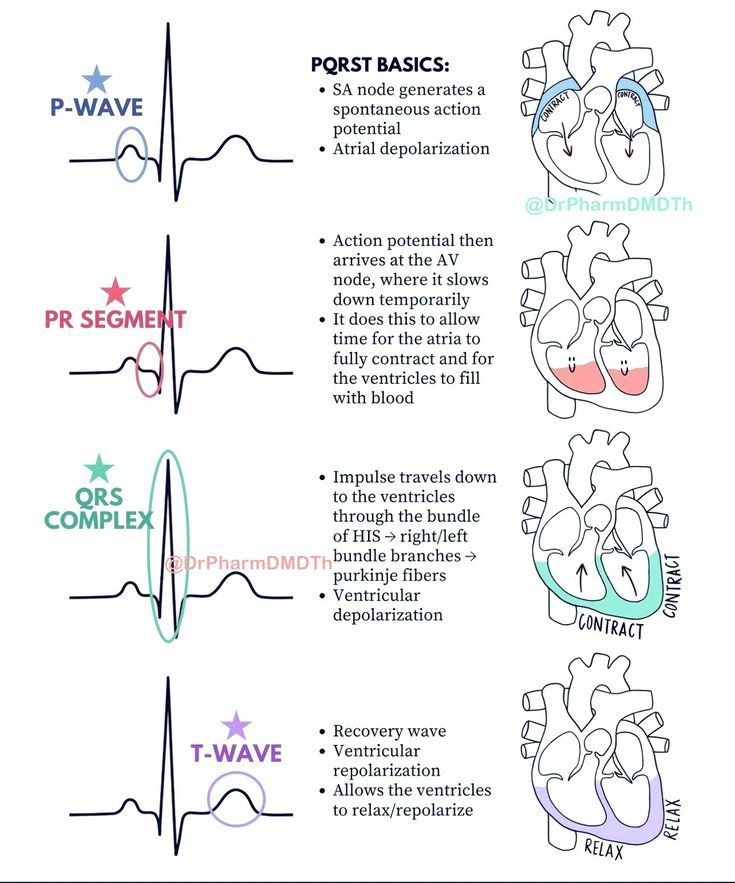
\includegraphics[width=0.4\textwidth]{3_Chapters/2_Chapter_LiteratureReview/Figures/PQRST_complex.jpg}
    \caption{Placeholder for ECG diagram}
    \label{fig:ECG_Waveform}
\end{figure}

The timing and amplitude of the PQRST wave are essential for patient health analysis \cite{Sinha2023SemiSupervisedCD}. Significant signal loss in the digisation process would thus render the ECG useless for diagnostic purposes.

The grid is formed ... such that reading the waveforms can remain consistent throughout.

\subsection{ECG leads}

The direction of this wave is dependent on the leads. The leads are defined by the electrodes used. In a 12-lead ECG, there are 10 electrodes used to measure the heart's activity from different angle and planes. Each lead provides different and vital information about arrhythmias and myocardial infarction (heart attacks). 

There are the limb electrodes places by the left arm and leg and the right arm. Measurements between two of them, with the third being a reference, creates the I, II, and III dipoles leads. When a fourth electrode known as the reference or zero electrode is introduced, the augmented leads are created. This is a measurement from one of the limb electrodes to the reference electrodes. This creates one of the unilateral leads. 

In 1934, it was noted that there were areas in the heart that needed to be measured to better detect myocardial infarctions. This gave birth to the precordial leads through the use of six electrodes placed around the precordial (chest area about and around the heart). 

These make up the 12 leads that illustrate the different waveform patterns seen in the electrocardiogram trace. They are used to section the ECG into 12 important regions which can be segmented and analysed further. \cite{AlGhatrif2012}

%----------------------------------------------------------------------------------------------

\section{Formats for Digitised ECGs}

In recent decades, multiple approaches have been developed for digitising and storing ECG records, ranging from the scanning of paper traces into PDF format to direct digitisation using computer applications such as MATLAB or Python.

\subsection{Scanned PDF Format}

The most straightforward method of digitising ECGs is by scanning paper records into PDF format. This approach makes data easily accessible across multiple devices, such as laptops and mobile phones. It also facilitates better organisation and storage of patient information, improving the efficiency of record retrieval and supporting long-term preservation that physical paper cannot guarantee.

However, this method has notable limitations. Since the ECG remains an image rather than raw signal data, it cannot be manipulated or re-analysed for further processing. Scanned records may contain physical defects such as creases, stains, or fading, particularly when dealing with older paper traces. These issues cannot be corrected during scanning, which reduces the reliability and quality assurance of the data. Thus, while efficient for archiving and accessibility, this approach is limited in its usefulness for future diagnostic and analytical applications.

\subsection{Manual Digitisation}

A more time-consuming approach to ECG digitisation involves manually recording the millivolt–time coordinates of the individual signal leads onto an electronic spreadsheet and entering them into software such as MATLAB or Python. Unlike scanning into PDF format, this method produces a true digital signal that can be manipulated, processed, and analysed with high accuracy. However, it is highly labour-intensive and susceptible to human error, particularly when large volumes of ECG records must be digitised.

\subsection{MATLAB/Python Digitisation}

Technological advancements, along with the development of Python and MATLAB libraries that integrate vision frameworks for object identification, have enabled the efficient extraction of signals from scanned ECG images. Algorithms can now automate the tracing of ECG waveforms into time-series coordinates, which can subsequently be plotted, analysed, and manipulated in digital form. The extracted data are typically stored in CSV format, facilitating efficient organisation, retrieval, and downstream processing.

This approach offers several advantages: automated signal acquisition, reliable digital storage through CSV files, and straightforward visualisation within environments such as MATLAB, Python IDEs, and Excel. Despite these benefits, practical limitations remain. Such tools are generally deployed on laptops or desktop computers, which may not always be accessible in the fast-paced environment of a hospital or outside clinical settings when records are urgently required. Furthermore, most implementations perform best with scanned images and often show reduced reliability when applied to camera-captured inputs, limiting their adaptability in resource-constrained or less controlled settings.

%-------------------------------------------------------

\section{Smartphone-based ECG Capturing}

\subsection{Performance - Resolution (can it handle it)}
%limitations can talk about camera resoluations - development
\subsection{Accessibility and Cost-Effectiveness}

%-------------------------------------------------------

\section{Digitisating ECG Signals}

The fundamental concept of digitising ECG signals lies heavily within image processing. Generally, the process involves preparing the image through filteration and artifact removal, isolating the region of interest, particularly the 12 leads, through segmentation, and converting the extracted ECG waveform into a one-dimensional digital signal suitable. However, machine learning models have also been used to achieve greater results in varying datasets. 

\subsection{Artifact Removal}
%method 1 - which is briefly ... method 2 - briefly ... (add in equations where possible/ table of comparison)
The report written by Cuong et al. highlights how the performance of their model dropped by 60.87\% when artifacts are present in the processed images \cite{Cuong2024}, emphasising the neeed for their removal.

\subsubsection{Shadow and Crease Removal}
%with grayscale ... with RGB (this is where I can add the RBG equation)
Shadows and creases represent the most disruptive artifacts in ECG image digitisation. Mishra et al. intorduces the concept of luminance correction for shadow removal, given that they occur due to obscured light \cite{Mishra2021}. This method involves changing the luminance/brightness of the \gls{ROI} without affecting the colour. This can me done in different colour spaces.

\begin{table}[H]
    \centering
	\caption{Luminance Correction Methods}\label{tab:lumcor}
    \begin{tabular}{|l|>{\raggedright\arraybackslash}p{4cm}|>{\raggedright\arraybackslash}p{3cm}|>{\raggedright\arraybackslash}p{3cm}|l|}
    \hline
    Space        & Description                                        & Strengths                           & Limitations                                       & Cite                 \\ \hline
    RGB          & Adjust luminance in  each channel           & Requires no conversion   & Can erode the colour                                  & \cite{Yang2022LABNetLC}  \\ \hline
    LAB          & Corrects luminance separately from colour   & Luminance and colour well separates & Can introduce noise                        & \cite{Yang2022LABNetLC}  \\ \hline
    YCbCr        & Corrects brightness separately from colour  & Good luminance separation           & Produces less uniform colour               & \cite{Wang2017StackedCG} \\ \hline
    \end{tabular}
\end{table}

\subsubsection{Noise Removal}
%different filters and their pros and cons (make it aplication based)

\textbf{Mean Filters:} Within a pixel cluster of odd nxn sizing, the middle pixel is replaced by the average of all their pixel values. It unfortunately serves to blur the image, removing important object detail \cite{Chauhan2018PerformanceAO}.\\
\textbf{Median Filters:} These are better capable at removing salt and pepper (discrete) noise, while preserving edge details. However, it does tend to remove finer details that appear as outliers in a cluster of pixels \cite{Chauhan2018PerformanceAO}.\\
\textbf{Gaussian Filters:} These better preserve finer details as compared to mean and median filters \cite{Chauhan2018PerformanceAO}. However, they perform poorly when applied to discrete noise.\\
\textbf{Wiener Filters:} In images that have noise caused by motion blur, these filter perform excellently. They are less effective for salt and pepper noise as compared to other linear filters \cite{Chauhan2018PerformanceAO}.

Camera-captured images are littered with continous random noise cause by the hardware involved. This makes filters that tackle Gaussian noise more appealing for the purpose of this project.

\subsubsection{Text Removal}

ECG papers contain labels for each lead. These characters need to be removed before converting the extracted wavform into a 1-D signal.

\textbf{Optical Character Recognition:} Vision frameworks are used to identify text in images. The algorithms than use morphological operators to isolate the regions, and image impairings to reconstruct the area \cite{Ganesh2021CombiningOC}.\\
\textbf{Image Processing:} There are a couple of image processing approaches that can be used to remove text, with most using cropping
\textbf{}

\subsection{Segmentation}
% separating to separate leads (use diagrams I generated in the benchmarking)

\subsubsection{Image Processing Approach}

\subsubsection{Machine Learning Approach}

%after both sections show a comparison table showing the pros and cons of each

\subsection{Background Removal and Signal Extraction}

\subsubsection{Image Processing Approach}

\subsubsection{Machine Learning Approach}

%after both sections show a comparison table showing the pros and cons of each

\subsection{Post-processing}
%Continuity (how it's detected) and what can be done to fix it

\subsection{Signal Digitisation}
%talk about consistency of the approach used, matbe highlight any slight differences in the implementation, use the equation form one of the reports

%-------------------------------------------------------

\section{Conclusion}

\begin{itemize}
    \item Summary of reviewed methods and gaps.
    \item Justification for proposed app.
    \item Key algorithmic challenges for this project.
\end{itemize}

% Literature Review
%\section{Literature Review}
\begin{itemize}
	\item{Broad description of subject}
	\item{Some relevant history}
	\item{Current implementations in industry}
	\item{New \& Related Research on the subject}
\end{itemize}